\documentclass[11pt,a4paper]{article}

\usepackage[T1]{fontenc}
\usepackage[utf8]{inputenc}
\usepackage[french]{babel}
\usepackage{lmodern}
\usepackage{geometry}
\usepackage{hyperref}
\usepackage{amssymb}
\usepackage{amsmath}
\usepackage{lmodern}
\usepackage{graphicx}
\usepackage{subcaption}
\usepackage[utf8]{inputenc}
\usepackage[T1]{fontenc}
\usepackage[french]{babel}
\usepackage{graphicx} % Indispensable pour insérer des images
\usepackage{geometry}

% Définition des marges
\geometry{margin=2.5cm}

\begin{document}

\begin{titlepage}
    \centering 
    

    
\includegraphics[height=2.5cm]{images/Logoum.png}
    \vspace{1cm} 
    \hspace{0.5cm} 
    
\includegraphics[height=2.5cm]{images/ssdlogo.png}
    
    \vspace{1.5cm}
    
    {\Large \textsc{MASTER II STATISTIQUES ET SCIENCES DES DONNÉES}}\\[0.5cm]
    {\large \textbf{Parcours Biostatistique}}
    
    \vspace{0.8cm}
    
    \rule{\linewidth}{0.5pt}
    \vspace{0.25cm}
    
    {\LARGE \textbf{ Identification des déterminants génétiques de la pathogénicité de la dengue\\[0.2cm]}}
    
    \vspace{0.25cm}
    \rule{\linewidth}{0.5pt}
    
    \vspace{1.2cm}
    
    \textbf{Présenté par :}\\
    Damien MARIAC\\[0.8cm]
    
    \textbf{Encadré par :}\\
    Vincent PEDERGNANA\\[0.8cm]

    \textbf{Tuteur FdS :}\\
    Ludovic Menneteau\\[0.8cm]

    \textbf{Jury :}\\
    Élodie BRUNEL-PICCININI\\
    Xavier BRY\\
    Benoite DE SAPORTA\\[1cm]
    
    \textbf{Année universitaire 2025-2026}
    
    \vfill
    

    
\includegraphics[height=3cm]{images/irdlogo.png} \hfill
    
\includegraphics[height=3cm]{images/mivegeclogo.png} \hfill
    
\end{titlepage}

\newpage
\tableofcontents

\newpage
\section{Environnement}
Bla bla sur la laboratoire et sur l'UMR MIVEGEC.

% 1 page NE PAS OUBLIER DE SUPPRIMER LE FICHIER AIDE
% Demander au tuteur de stage si je peux mettre ma participation au financement d'une ED.

% Re aligner avec le virus H77 NCBI

% 5.4 application sur le jeu de la DENV

% Perspective thèSE = nouveau codage (profondeur)

% Gamma lien  ;

\newpage
\section{Context}
\subsection{Context du sujet}
D'un individus à un autre, les symptômes d'une infection virale peuvent varier allant d'une absence de symptômes à des formes sévères.
Cette variabilité est en partie due à la diversité génétique de l'hôte et du virus.
L'objectif de cette étude est de proposer de nouveaux modèle permettant de faciliter l'étude d'associations entre les variants génétiques de l'hôte et les mutations virales, afin de mieux comprendre les mécanismes des réponses immunitaires.
\\
\\
Historiquement, les études d'association sont menées sur les symptomes eux mêmes. Mais ceux-ci sont souvent largement influencés par des facteurs tel que l'environnement, l'alimentation ou les habitudes physique. 
\\
\\
Il existe depuis quelques années une variante de cette approche qui consiste à considerer le code génétique du virus comme symptome. L'idée est que les mutations virales sont le reflet de la pression de sélection exercée par le système immunitaire de l'hôte. Ainsi, en identifiant les variants génétiques de l'hôte associés à certaines mutations virales, on peut obtenir des informations sur les mécanismes immunitaires impliqués dans la réponse à l'infection.
\\
\\
Ce qui fait toute la difficulté de cette approche est la haute dimensionnalité des données. En effet, on a du côté des hôtes des centaines de milliers de variants génétiques et du côté des virus des centaines de mutations après avoir filtré les sites dépassant un certain taux de variabilité.
\\
De plus, les individus issus de régions géographiques et d'ethnies différentes présentent des différences génétiques ce qui biaisent les résultats d'association. Il est donc nécessaire de prendre en compte la structure de population des hôtes.
Mais il est également nécessaire de prendre en compte la structure de population des virus. En effet, les virus issus d'une même région géographique ou d'une même lignée évolutive partagent des mutations communes. Il est donc nécessaire de prendre en compte la structure de population des virus.

\subsection{Context biologique}

Le virus est une entité biologique qui ne peut pas se reproduire par elle-même. Il a besoin d'un hôte pour se multiplier et se propager. Il est constitué d'une coque qui protège son matériel génétique, qui peut etre de l'ADN ou de l'ARN.
La nature du support de l'information ADN ou ARN dicte la réplication, ce qui a un impact majeur sur sa diversité génétique. De ce fait, les virus à ARN ont un taux de mutation beaucoup plus élevé que les virus à ADN.
Cela est dû au fait que l'ARN polymérase, l'enzyme responsable de la réplication de l'ARN, n'a pas de mécanisme de correction d'erreurs contrairement à l'ADN polymérase. Cette haute variance est fondamentale : elle permet au virus de s'adapter très rapidement pour trouver des solutions face aux défenses de l'hôte.
\\
\\
Dans le cadre de ce stage, nous avons travaillé sur le virus de l'hépatite C dont on a déjà identifié des liaisons afin de pouvoir l'étendre sur le virus de la dengue. Ce sont tous deux des virus à ARN qui présentent une grande diversité génétique.

\subsection{Extraction des données}


\newpage
\section{Préparation des données}

\subsection{Alignement}

\subsection{Traitement des valeurs manquantes}


\newpage
\section{Modélisation statistique}

% expliquer pourquoi un modèle supervisé est nécessaire pour ce type de données

\subsubsection{Modèle d'association ``classique''}

Le modèle proposé par \cite{ref1} vise à modéliser la probabilité d'une mutation
virale en fonction d'un SNP de l'hôte et de covariables telles que l'âge et le
sexe. Pour un site viral et un SNP donnés, une régression logistique est ajustée
indépendamment, et ce pour l'ensemble des paires SNP--site viral.

Afin de corriger la structure de population, les auteurs incluent les composantes
principales (CP) de l'hôte et du virus comme effets fixes. En effet, les
premières CP de l'hôte capturent l'origine ethnique des individus \cite{ref2},
et les premières CP du virus capturent l'origine géographique des souches
\cite{ref3} (Figure~\ref{fig:acp}).


% REFAIRE GRAPH
\begin{figure}[htbp]
    \centering
    \begin{subfigure}[b]{0.49\textwidth}
        \centering
        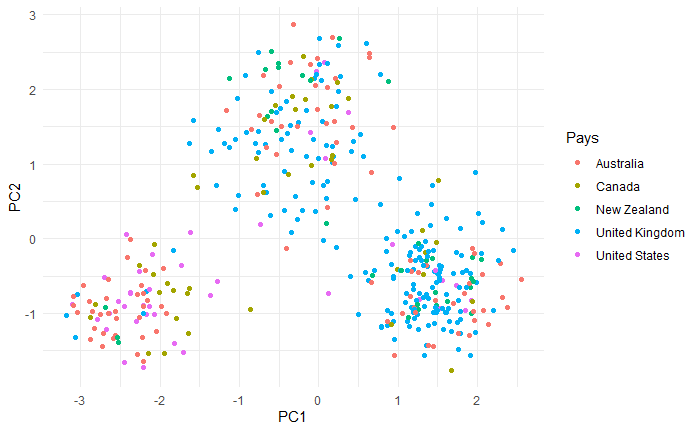
\includegraphics[width=\textwidth]{images/ACPvirusall.png}
        \caption{PC1 et PC2 du virus, par pays}
        \label{fig:acp-virus}
    \end{subfigure}
    \hfill
    \begin{subfigure}[b]{0.5\textwidth}
        \centering
        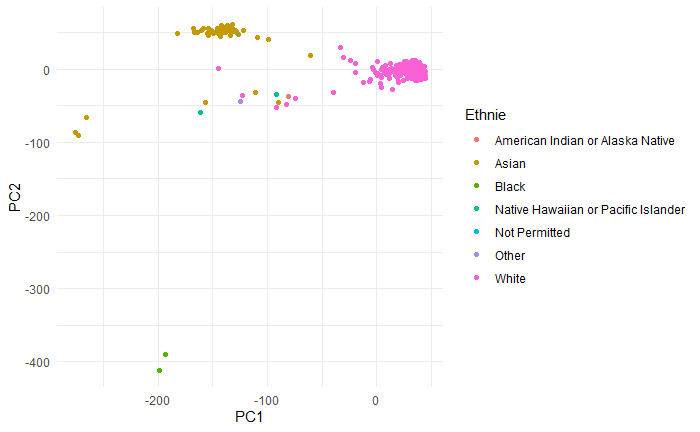
\includegraphics[width=\textwidth]{images/ACPhoteall.png}
        \caption{PC1 et PC2 de l'hôte, par ethnie}
        \label{fig:acp-hote}
    \end{subfigure}
    \caption{Structure de population capturée par l'ACP.}
    \label{fig:acp}
\end{figure}

Les auteurs retiennent les 10 premières CP de l'hôte et les 5 premières du
virus. Ce choix reste discutable : ces composantes ne capturent respectivement
que XX\,\% et 12\,\% de la variance cumulée, ce qui suggère qu'une part
importante de la structure de population n'est pas corrigée.

Le modèle s'écrit finalement, pour un SNP $j$ et un site viral $i$ fixés :
\[
\text{logit}\big(P(Y_i = 1)\big) = \beta_0 + \beta_{ij}\, SNP_j
+ \sum_{k=1}^{10} \gamma_k\, PC^{h\^ote}_k + \sum_{l=1}^{5} \delta_l\, PC^{virus}_l
\]

Une p-value est extraite pour chaque test SNP--site viral. Les tests étant
menés indépendamment sur un très grand nombre de paires, une correction pour
tests multiples est nécessaire afin de limiter les faux positifs : les
auteurs utilisent une correction de Bonferroni, avec un seuil de
significativité $\alpha = 10^{-8}$.


Afin de pouvoir représenter les résultats, on peut construire un \textit{Manhattan plot}.
Celui-ci est un graphique qui représente les p-values de chaque SNPpour un site viral donné.

\begin{figure}[h!]
    \centering
    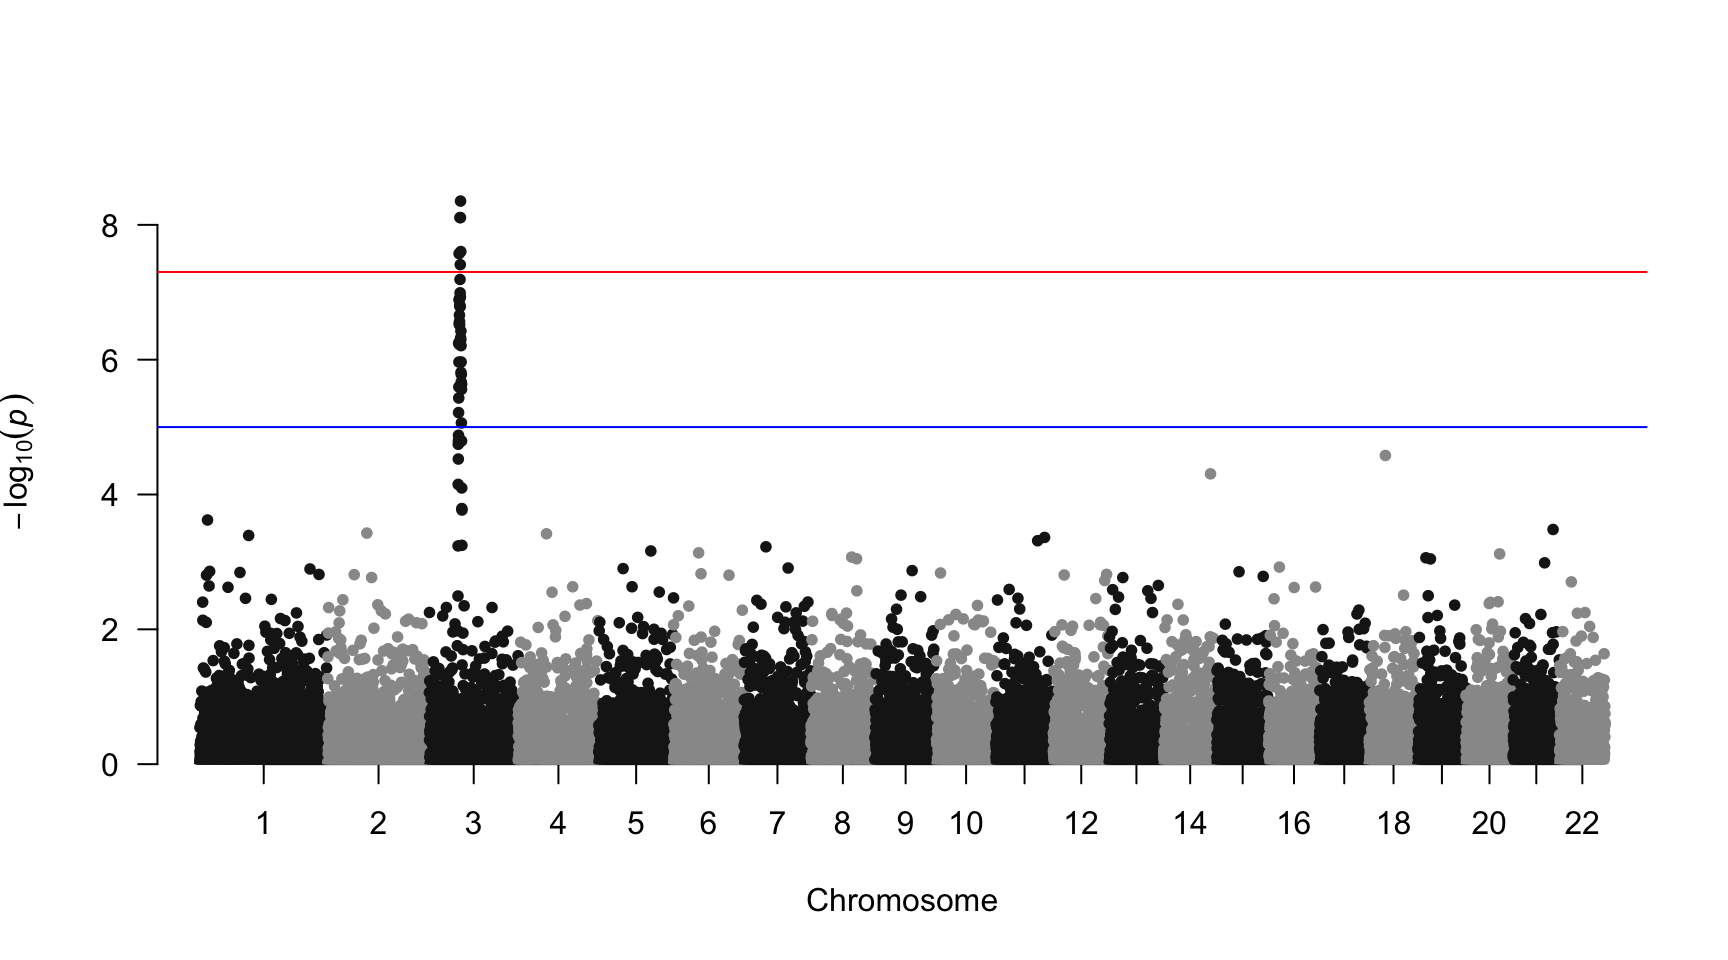
\includegraphics[width=\textwidth]{images/manhattanplot.png}
    \caption{Manhattan plot pour un site viral donné.}
    \label{fig:manhattan}
\end{figure}

\newpage
\subsubsection{Limites du modèle ``classique''}

Ce modèle présente plusieurs limites ce qui motivent le développement d'une
approche plus adaptée à ce type de données.

D'abord, il ne capture qu'une fraction de la structure de population : se
limiter à quelques composantes principales, en plus d'ignorer une part
importante de la variance, ne permet pas de représenter plus précisément la
dépendance génétique entre individus (côté hôte) ou entre souches (côté
virus).

Ensuite, il ignore la corrélation entre sites : les mutations virales peuvent
être corrélées entre elles du fait de leur proximité structurale
(conformation 3D de la protéine), et les SNPs de l'hôte proches sur le génome
sont corrélés par déséquilibre de liaison. Ne pas modéliser ces dépendances
revient à traiter chaque test comme indépendant alors qu'il ne l'est pas,
ce qui biaise l'estimation de la significativité.

Puis, la correction de Bonferroni, en supposant l'indépendance des tests,
est très conservatrice dans ce contexte de forte corrélation : elle risque
d'écraser un signal réel, en particulier étant donné la très haute
dimensionnalité des données (des millions de tests SNP--site viral).
  
\vspace{0.5cm}

\subsection{Modèle avec dépendances : Graph Fused Lasso}

Un modèle de type Graph Fused Lasso (GFL) permettrait de pouvoir palier au problème de la corrélation entre sites.
Celui-ci reprend le modèle logistique
précédent, mais ajoute deux pénalisations sur les coefficients
$\beta_{ij}$~: une pénalité de type Lasso, qui contraint les coefficients à
être nuls si le SNP $j$ n'est pas suffisamment associé au site viral $i$, et
une pénalité de fusion sur graphe, qui contraint les coefficients à être
similaires lorsque les sites viraux $i$ et $i'$ sont corrélés.

Le modèle s'écrit alors, pour un SNP $j$ fixé :
\[
\hat{\boldsymbol{\beta}}_{\cdot j} = \operatorname*{argmin}_{\boldsymbol{\beta}_{\cdot j}}
\left\{ -\sum_{i=1}^{p} \ell_i(\beta_{ij}) 
+ \lambda_1 \sum_{i=1}^{p} |\beta_{ij}|
+ \lambda_2 \sum_{(i,i') \in E} w_{ii'} \, |\beta_{ij} - \beta_{i'j}| \right\}
\]

où $\ell_i(\beta_{ij})$ est la log-vraisemblance logistique associée au site
viral $i$, $E$ l'ensemble des arêtes du graphe de corrélation entre sites
viraux, $w_{ii'}$ le poids de l'arête reliant les sites $i$ et $i'$, et
$\lambda_1$, $\lambda_2$ les paramètres de régularisation contrôlant
respectivement la sparsité et l'homogénéité locale des coefficients sur le
graphe.

\subsubsection{Construction du graphe de corrélation}

Afin d'implémenter ce modèle, il est nécessaire de construire un graphe
représentant les corrélations entre sites viraux. Les sites viraux étant
binaires, ils sont supposés suivre une loi de Bernoulli, ce qui permet
d'estimer leur corrélation de façon paramétrique. Pour deux sites viraux $i$
et $i'$, de probabilités marginales $p_i$ et $p_{i'}$ et de probabilité
jointe $p_{ii'} = P(Y_i = 1, Y_{i'} = 1)$, la corrélation s'écrit :
\[
w_{ii'} = \text{corr}(Y_i, Y_{i'}) = 
\frac{p_{ii'} - p_i \, p_{i'}}{\sqrt{p_i (1-p_i)\, p_{i'} (1-p_{i'})}}
\]

La matrice de corrélation ainsi obtenue sert de support au graphe~: une
arête est créée entre deux sites viraux lorsque leur corrélation dépasse un
seuil fixé. La Figure~\ref{fig:heatmap}
représente cette matrice sous forme de heatmap, où les valeurs proches de 1
sont en rouge et celles proches de 0 en jaune.


\begin{figure}[h!]
    \centering
    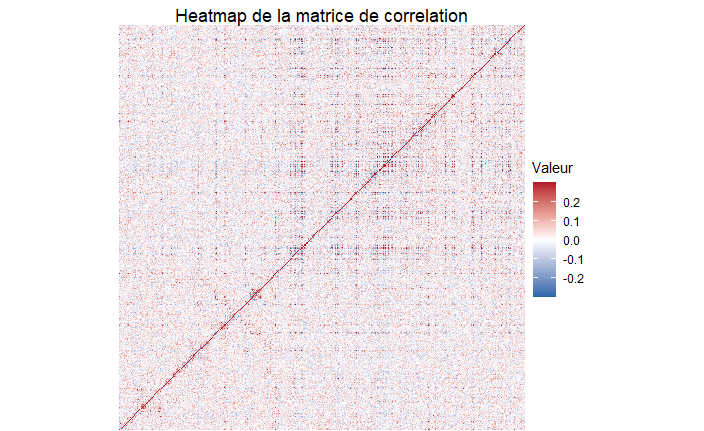
\includegraphics[width=\textwidth]{images/heatmapcorr.png}
    \caption{Matrice de corrélation entre sites viraux sous forme de heatmap.}
    \label{fig:heatmap}
\end{figure}


\subsubsection{Choix des paramètres de régularisation}

Il reste à définir les paramètres de régularisation $\lambda_1$ et
$\lambda_2$. Une validation croisée sur l'ensemble des données étant
impossible à mettre en œuvre dans ce contexte de très haute dimensionnalité,
elle a été réalisée sur plusieurs sous-ensembles de données, et les résultats
ont ensuite été moyennés pour obtenir les paramètres optimaux. On obtient
ainsi $\lambda_1 = XX$ et $\lambda_2 = XX$.

\subsubsection{Optimisation du modèle : algorithme FISTA}

L'estimation des coefficients du modèle revient à minimiser la fonction
objectif présentée précédemment, qui se décompose en une partie lisse et une
partie non lisse :
\[
F(\boldsymbol{\beta}) = \underbrace{f(\boldsymbol{\beta})}_{\text{log-vraisemblance logistique}}
+ \underbrace{g(\boldsymbol{\beta})}_{\text{pénalités}}, \qquad
g(\boldsymbol{\beta}) = \lambda_1 \sum_{i=1}^{p} |\beta_{ij}|
+ \lambda_2 \sum_{(i,i') \in E} w_{ii'} \, |\beta_{ij} - \beta_{i'j}|
\]

où $f$ est convexe et différentiable, mais où $g$ est convexe et non
différentiable en raison des valeurs absolues. Cette fonction ne possède pas
de solution analytique et doit donc être minimisée numériquement.

Pour cela, nous utilisons l'algorithme FISTA (Fast Iterative
Shrinkage-Thresholding Algorithm) \cite{ref4}, particulièrement adapté aux
problèmes de la forme $\min_{\boldsymbol\beta} f(\boldsymbol\beta) +
g(\boldsymbol\beta)$ lorsque $f$ est différentiable à gradient
$L$-Lipschitzien et $g$ admet un opérateur proximal calculable. C'est la
méthode principalement utilisée dans les packages R qui implémentent les
modèles de type Lasso.

\vspace{1cm}

\paragraph{Étape de descente de gradient.}
À chaque itération $k$, l'algorithme réalise d'abord un pas de gradient sur
la partie lisse $f$, évalué non pas en $\boldsymbol\beta_k$ mais en un point
extrapolé $\mathbf{y}_k$ :
\[
\mathbf{z}_k = \mathbf{y}_k - \frac{1}{L} \nabla f(\mathbf{y}_k)
\]
où $\nabla f(\mathbf{y}_k)$ est le gradient de la log-vraisemblance
logistique, de la forme $\mathbf{X}^\top (\mathbf{p}(\mathbf{y}_k) -
\mathbf{Y})$, avec $\mathbf{p}(\mathbf{y}_k)$ le vecteur des probabilités
prédites $\text{logit}^{-1}(\mathbf{X}\mathbf{y}_k)$, et $L$ une constante de
Lipschitz du gradient (majorée ici par la plus grande valeur propre de
$\mathbf{X}^\top \mathbf{X}/4$), qui fixe la taille du pas.

\paragraph{Étape de seuillage (opérateur proximal).}
Le point $\mathbf{z}_k$ est ensuite projeté via l'opérateur proximal de $g$,
défini par :
\[
\text{prox}_{g/L}(\mathbf{z}_k) = \operatorname*{argmin}_{\boldsymbol\beta}
\left\{ \frac{L}{2} \lVert \boldsymbol\beta - \mathbf{z}_k \rVert_2^2 +
g(\boldsymbol\beta) \right\}
\]
Pour la seule pénalité $\ell_1$, cet opérateur a une solution explicite, le
seuillage doux (\textit{soft-thresholding}) :
\[
\big[\text{prox}_{\lambda_1/L \, \lVert \cdot \rVert_1}(z)\big]_i
= \text{sign}(z_i) \, \max\big(|z_i| - \lambda_1/L,\; 0\big)
\]
qui annule progressivement les coefficients de faible amplitude, ce qui
permet de sélectionner uniquement les mutations virales les plus associées
au SNP étudié. En présence de la pénalité de fusion sur graphe, l'opérateur
proximal combiné $\text{prox}_{g/L}$ n'a plus de forme close et est résolu
par %\textcolor{red}{[préciser : solveur dédié / ADMM interne / dual path  algorithm, selon votre implémentation]}.

\paragraph{Étape d'accélération.}
Enfin, FISTA ajoute une étape d'extrapolation de type Nesterov, en combinant
les deux dernières estimations $\boldsymbol\beta_k$ et
$\boldsymbol\beta_{k-1}$ :
\[
\boldsymbol\beta_k = \text{prox}_{g/L}(\mathbf{z}_k), \qquad
t_{k+1} = \frac{1 + \sqrt{1 + 4 t_k^2}}{2}, \qquad
\mathbf{y}_{k+1} = \boldsymbol\beta_k + \frac{t_k - 1}{t_{k+1}}
\left(\boldsymbol\beta_k - \boldsymbol\beta_{k-1}\right)
\]
avec $t_1 = 1$ et $\mathbf{y}_1 = \boldsymbol\beta_0$. Cette accélération
permet d'obtenir une vitesse de convergence en $\mathcal{O}(1/k^2)$, contre
$\mathcal{O}(1/k)$ pour l'algorithme ISTA classique (sans extrapolation),
tout en conservant une implémentation relativement simple. Cette propriété
est particulièrement intéressante dans notre contexte, où le modèle doit
être estimé pour un très grand nombre de SNPs et de sites viraux.

\vspace{1cm}

Cepandant, dans le contexte de très haute dimensionnalité des données, l'algorithme FISTA
met un temps de calcul très long pour converger.
\\
\\
En effet, après avoir testé sur un sous-ensemble de données afin de pouvoir estimer 
le temps d'implémentation sur l'ensemble des données, on a pu constater un temps de calcul
de plusieurs mois pour l'ensemble du jeu de données.
\\
\\
De plus, l'algorithme FISTA ne peut pas être parallélisé du à la dépendance entre les sites qui impose de calculer les coefficients simultanément.
\\
\\
Il est donc nécessaire de trouver une alternative à cette approche afin de pouvoir estimer le modèle sur l'ensemble des données.

\vspace{1cm}

\subsection{Modèle avec effets aléatoires}

Le modèle GFL présenté précédemment permet de prendre en compte la
corrélation locale entre sites, mais uniquement via un graphe construit.
Il ne modélise pas la structure globale de
parenté génétique au sein des populations hôte et virale, pourtant décrite
comme un facteur de confusion majeur dans les études d'interaction
génome-à-génome \cite{fellay2020}. Une approche alternative, largement
utilisée dans les études d'association (GWAS) classiques,
consiste à modéliser cette structure via des \textbf{effets aléatoires},
plutôt que par un nombre limité de composantes principales ou un graphe de
corrélation. Cette stratégie a notamment été adaptée dans un contexte similaire par
\cite{...} au travers de la méthode ATOMM (\textit{Adaptive Two-way Mixed Model}),
qui introduit un effet aléatoire distinct pour l'hôte et pour le virus.



En reprenant cette idée, le modèle logistique s'écrit alors comme un modèle
mixte linéaire généralisé (GLMM) à deux effets aléatoires :
\[
\text{logit}\big(P(Y_i = 1)\big) = \beta_0 + W\alpha + X_j \beta_{ij}
+ \eta_v + \eta_h
\]
où $W\alpha$ regroupe les effets fixes (covariables telles que l'âge ou le
sexe), $X_j \beta_{ij}$ représente l'effet du SNP $j$ sur le site viral $i$,
et les deux effets aléatoires
\[
\eta_v \sim \mathcal{N}(0, \sigma^2_v K_v), \qquad
\eta_h \sim \mathcal{N}(0, \sigma^2_h K_h)
\]
capturent respectivement la structure de parenté génomique du virus et de
l'hôte, via les matrices de parenté génomique $K_v$ et $K_h$.
\\
Contrairement aux composantes principales, ces matrices résument l'intégralité de la
similarité génétique entre individus (ou souches), sans perte d'information
liée à un nombre de dimensions fixé a priori.

Dans ce cadre, l'intérêt principal n'est plus seulement d'estimer les
coefficients du modèle, mais de tester la significativité de
l'association entre chaque SNP de l'hôte $j$ et chaque site viral $i$,
c'est-à-dire tester "$H_0 : \beta_{ij} = 0$". Or, ce test doit être répété
pour un très grand nombre de paires SNP--site viral, et une estimation
classique du modèle par maximum de vraisemblance nécessiterait de réinverser
la matrice de covariance globale à chaque test, ce qui est numériquement
impossible à l'échelle de nos données. Il est donc nécessaire d'utiliser une
méthode d'estimation factorisée, qui sépare l'estimation des paramètres de
nuisance (communs à tous les tests) de celle du test d'association
lui-même : le test du score de Rao.

\vspace{1cm}

\subsubsection{Estimation - Test du score de Rao}

L'évaluation de chaque paires de variants (hôte, virus) implique d'ajuster le modèle mixte des millions de fois. Or, l'estimation des composantes de la variance ($\sigma^2_v$, $\sigma^2_h$) par maximum de vraisemblance nécessite l'inversion répétée de matrices de grande dimension, ce qui représente un coût computationnel important.
\\
\\
Concrètement, la procédure se déroule en deux étapes :
\begin{enumerate}
    \item \textbf{Ajustement sous $H_0$} : On force le coefficient d'intérêt $\beta_{ij}$ à $0$. Le modèle nul ne contenant que l'intercept, les covariables et les effets aléatoires est ajusté une seule fois par phénotype viral pour estimer les paramètres de nuisance et les composantes de la variance.
    \item \textbf{Calcul du score} : Pour chaque variant de l'hôte $j$, on évalue le gradient de la log-vraisemblance au point $\beta_{ij} = 0$. Si ce gradient est significativement éloigné de zéro, l'hypothèse nulle est rejetée, indiquant une association entre $X_j$ et $Y_i$.
\end{enumerate}

Cette méthode permet d'éviter le réajustement des effets aléatoires pour chaque SNP testé, réduisant ainsi drastiquement la complexité algorithmique tout en conservant une grande robustesse statistique.
\\
\\
La contre partie de ce test est qu'il ne fournit pas d'estimation directe de l'effet $\beta_{ij}$, mais uniquement une statistique de test et une p value associée. Cependant, dans le contexte d'une étude exploratoire visant à identifier des associations potentielles, cette limitation est acceptable.
\\
Néanmoins, pour les associations les plus prometteuses, il est possible de réajuster le modèle complet afin d'obtenir des estimations précises des effets et de leurs intervalles de confiance.
\\
\\
Il existe quand même des façons d'obtenir une estimation de l'effet $\beta_{ij}$ à l'aide des p-values. % à completer car je ne m'en souviens plus

\vspace{1cm}
\newpage
\section{Résultats et discussion}
\subsection{Choix du codage}
\subsection{Comparaison des modèles}
\subsection{Performances du modèle retenu}


\newpage
\section{Conclusion et perspectives}


\newpage
\section{Annexes}
\subsection{Annexe 1}

\newpage
\section{Bibliographie}



\end{document}